\documentclass{beamer}

\usepackage[utf8]{inputenc}
\usepackage{beamerthemesplit}
\usepackage{url}
\usepackage{hyperref}
\usepackage{tikz}
\usepackage{alltt}

\usepackage{listings}
\usepackage{marvosym}
\usepackage{color}
\usepackage[multidot]{grffile}
\usepackage{multirow}
\usepackage{array}
\usepackage{setspace}

\usepackage{CJKutf8}
\newcommand{\zhs}[1]{\begin{CJK}{UTF8}{gbsn}#1\end{CJK}}

\usetheme{Madrid}

\usecolortheme[RGB={132,186,75}]{structure}
\definecolor{cactusgreen}{RGB}{132,186,75}
\newcommand{\red}[1]{\textcolor{cactusgreen}{#1}}
\newcommand{\black}[1]{\textcolor{black}{#1}}

\graphicspath{{../pics/}}

\logo{
\includegraphics[height=0.7cm]{CLR_HOR}} 

\newcommand{\head}[2]
 {\frame{\frametitle{}\begin{centering}\LARGE#1\\#2\end{centering}}}

\newcommand{\abspic}[4]
 {\vspace{ #2\paperheight}\hspace{ #3\paperwidth}\includegraphics[height=#4\paperheight]{#1}\\
  \vspace{-#2\paperheight}\vspace{-#4\paperheight}\vspace{-0.0038\paperheight}}

\newcommand{\picw}[4]{{
 \usebackgroundtemplate{
 \color{black}\vrule width\paperwidth height\paperheight\hspace{-\paperwidth}\hspace{-0.01\paperwidth}
 \hspace{#4\paperwidth}\includegraphics[width=#3\paperwidth, height=\paperheight]{#1}}\logo{}
 \frame[plain]{\frametitle{#2}}
}}
\newcommand{\pic}[2]{\picw{#1}{#2}{}{0}}

\newcommand{\question}[1]{\frame{\begin{centering}\Huge #1\\\end{centering}}}
\newcommand{\redidot}{\makebox[0mm]{\hphantom{i}\red{i}}{\i}}
\newcommand{\blackidot}{\makebox[0mm]{\hphantom{i}\black{i}}{\i}}

% We want to use the infolines outer theme because it uses so less space, but
% it also tries to print an institution and the slide numbers
% Therefore, we here redefine the footline ourselfes - mostly a copy & paste from
% /usr/share/texmf/tex/latex/beamer/themes/outer/beamerouterthemeinfolines.sty
\defbeamertemplate*{footline}{infolines theme without institution and slide numbers}
{
  \leavevmode%
  \hbox{%
  \begin{beamercolorbox}[wd=.25\paperwidth,ht=2.25ex,dp=1ex,center]{author in head/foot}%
    \usebeamerfont{author in head/foot}\insertshortauthor
  \end{beamercolorbox}%
  \begin{beamercolorbox}[wd=.5\paperwidth,ht=2.25ex,dp=1ex,center]{title in head/foot}%
    \usebeamerfont{title in head/foot}\insertshorttitle
  \end{beamercolorbox}%
  \begin{beamercolorbox}[wd=.25\paperwidth,ht=2.25ex,dp=1ex,center]{date in head/foot}%
    \usebeamerfont{date in head/foot}\insertshortdate{}
  \end{beamercolorbox}}%
  \vskip0pt%
}
% No navigation symbols
\setbeamertemplate{navigation symbols}{}

\title[Working with Jupyter]{Working with Jupyter}
\author[Steven Brandt]{and Steven R. Brandt}
\institute{Center for Compuation and Technology\\
 Louisiana State University\\
 Funded by: NSF OAC 1550551}
\titlegraphic{
 
\includegraphics[height=2cm]{cactuslogo}\\
}
\date[2017-07-31]{2017-07-31}

\begin{document}

\frame{\titlepage}

\frame{\frametitle{What is Jupyter}
{\huge What is Jupyter?}
\begin{itemize}
\item \textbf{A Notebook} Jupyter provides notebook-style access to running code in any language (It's name is a mashup of Julia, Python, and R).
\item \textbf{An Executable Paper} Jupyter allows its creator to mix code, the results of execution,
images, and arbitrary markeup to be combined in a document that is both a paper and code.
\item \textbf{A New Way to Interact} Jupyter is a new way to interact with a set of calculations.
\begin{itemize}
\item It is neither a gui nor a command-line interface, but a combination of both. 
\item It is intended to be interactive and dynamic, but it is readable and useful in static form.
\end{itemize}
\end{itemize}
}

\frame{\frametitle{Your Jupyter Notebook}
\begin{itemize}
\item For this workshop, we are going to be using
an NCSA machine called Nebula (http://www.etk2017.ndslabs.org/).
\item The above is a virtual machine based on Docker. If you want
to run the Docker image directly on your laptop instead of the class
machine, you can obtain it like this: ``docker pull craigwillis/jupyter-et''
and you can run it  like this ``docker run -it -habc-jupyteret-def -p 8000:8000 --user 1000 craigwillis/jupyter-et jupyter notebook --port 8000 --ip 0.0.0.0 --no-browser'' That will start jupyter on port 8000.
You can pick a different port if you like.
\item If anything should go wrong with this machine, we have a backup
located at LSU (http://hpx-jupyter.cct.lsu.edu)
\item Navigate to the first link now.
\end{itemize}
}

\frame{\frametitle{Your Jupyter Notebook}
Click ``Sign in here'' then launch your ``Jupyter/Einstein Toolkit'' macine instance.

\begin{centering}
  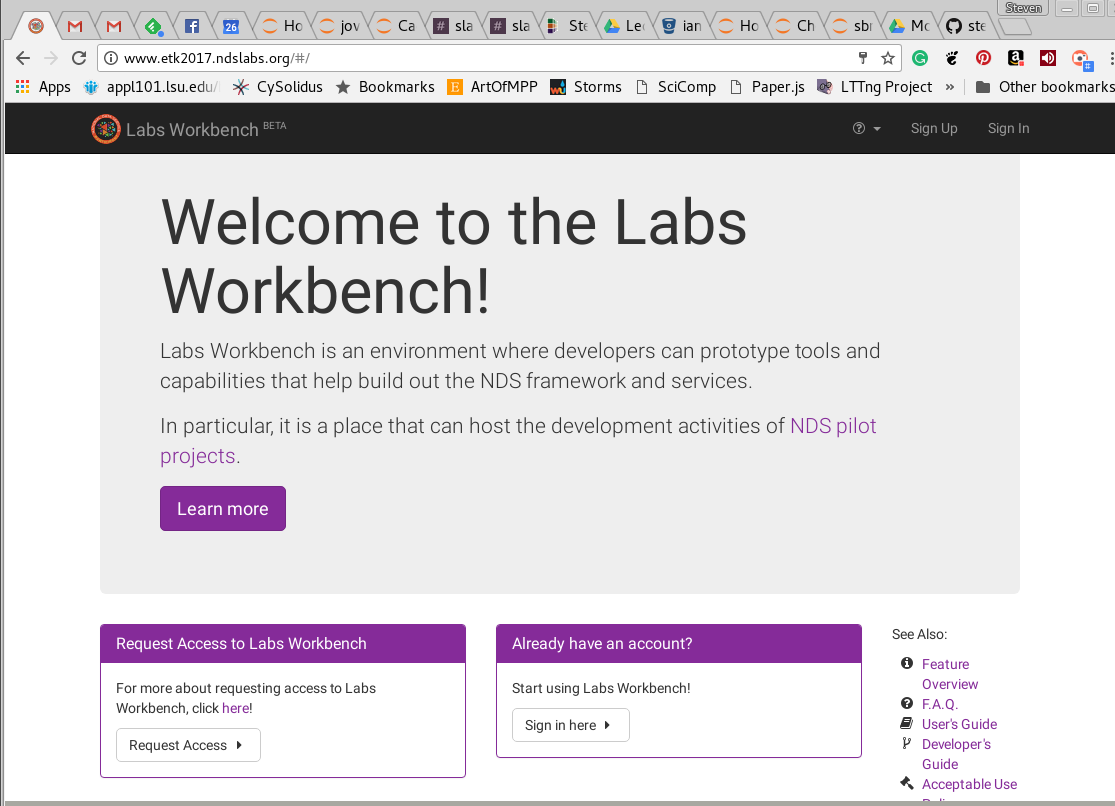
\includegraphics[height=0.45\textwidth]{signin}\\
\end{centering}
}

\frame{\frametitle{Your Jupyter Notebook}
Next, launch your machine instance.

\begin{centering}
  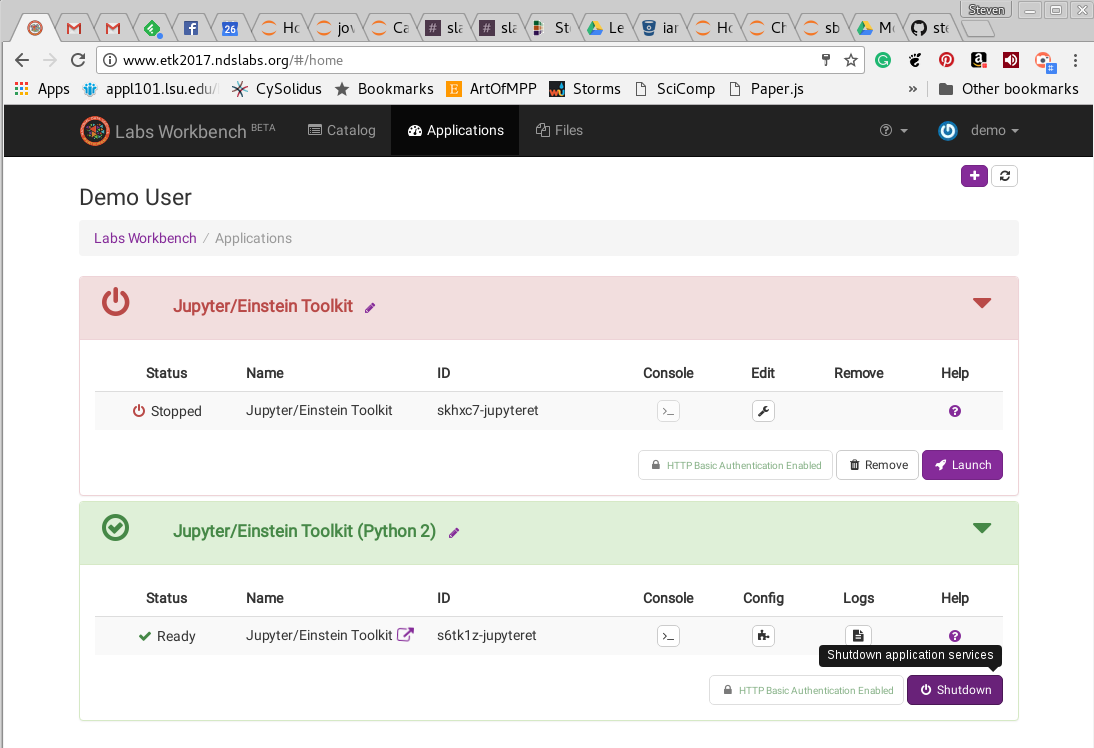
\includegraphics[height=0.45\textwidth]{launch}\\
\end{centering}
}

\frame{\frametitle{Your Jupyter Notebook}
In addition to the notebook, the Jupyter interface provides you with a fully functioning terminal.
Please open one now.

\begin{centering}
  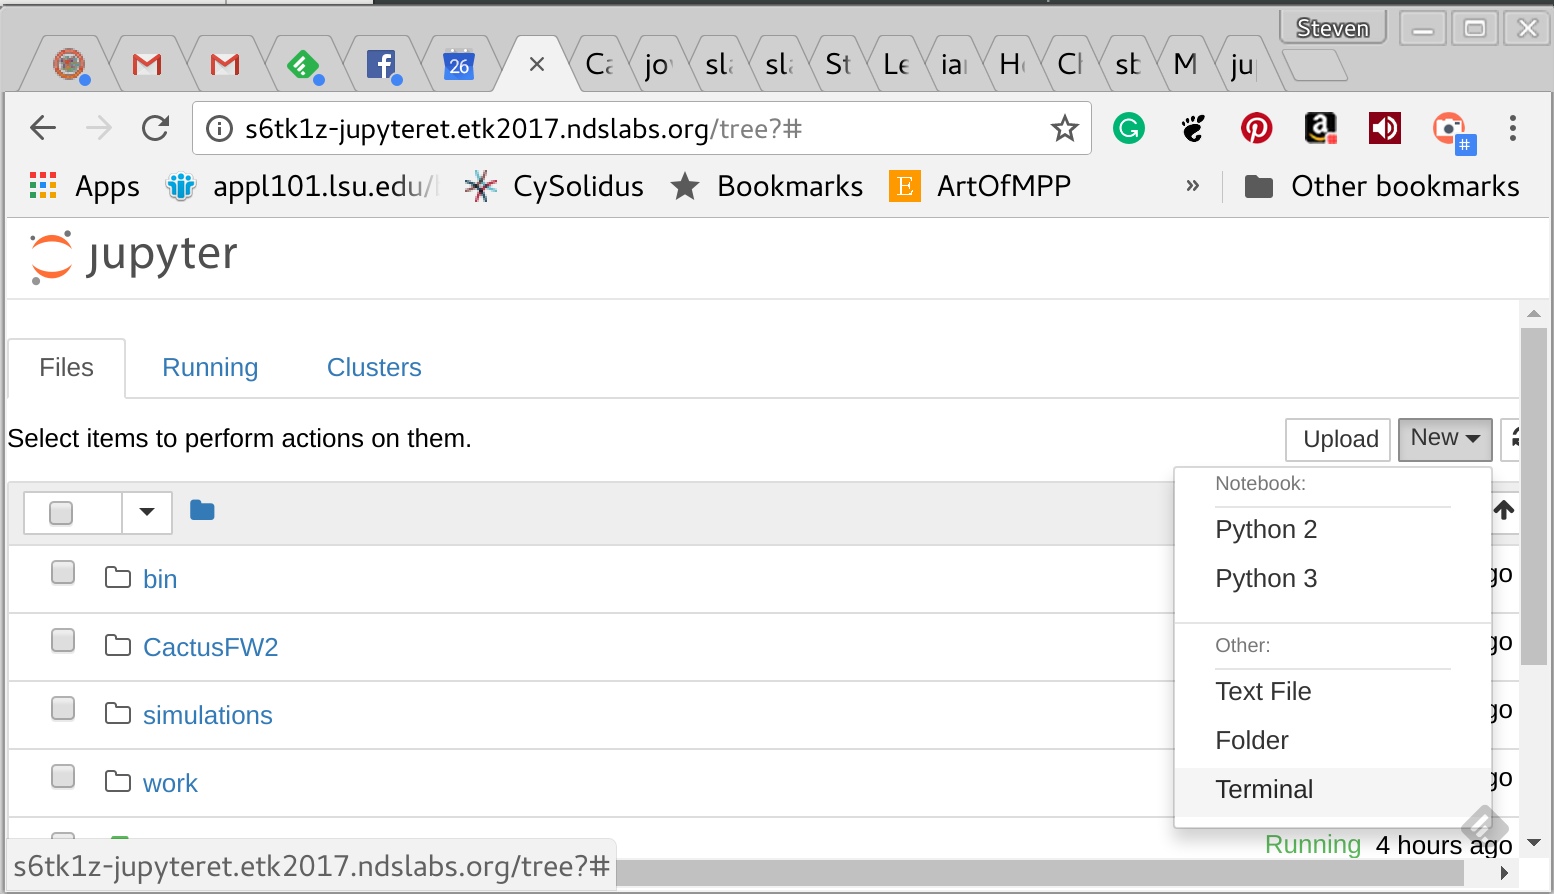
\includegraphics[height=0.45\textwidth]{terminal}\\
\end{centering}

Some things are still easier outside the notebook.
}

\frame{\frametitle{Your Jupyter Notebook}
Now, log into nebula, open a terminal, and type the
command\\ ``git clone https://github.com/stevenrbrandt/CactusTutorial.git''

\begin{centering}
  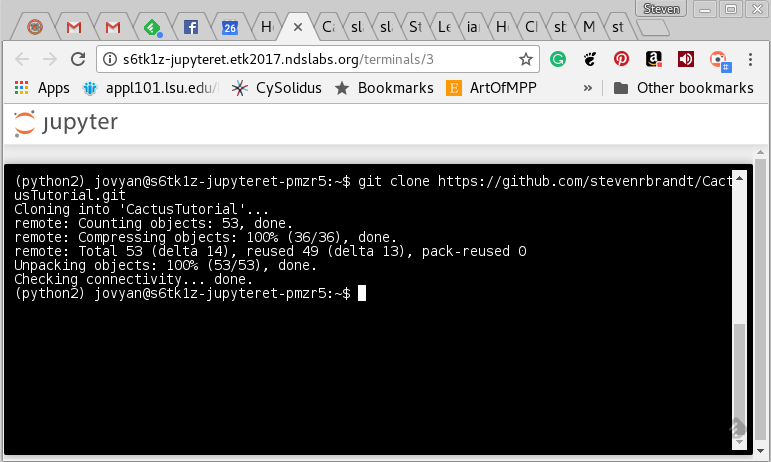
\includegraphics[height=0.45\textwidth]{clone}\\
\end{centering}
}

\frame{\frametitle{Your Jupyter Notebook}
Open the tutorial from within Jupyter

\begin{centering}
  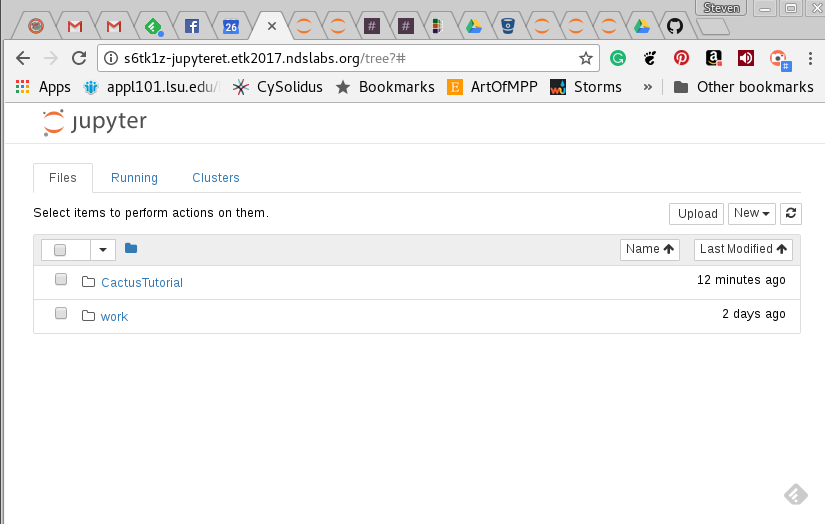
\includegraphics[height=0.45\textwidth]{opentut}\\
\end{centering}
}

\frame{\frametitle{Your Jupyter Notebook}
Open the numerical methods folder from within Jupyter

\begin{centering}
  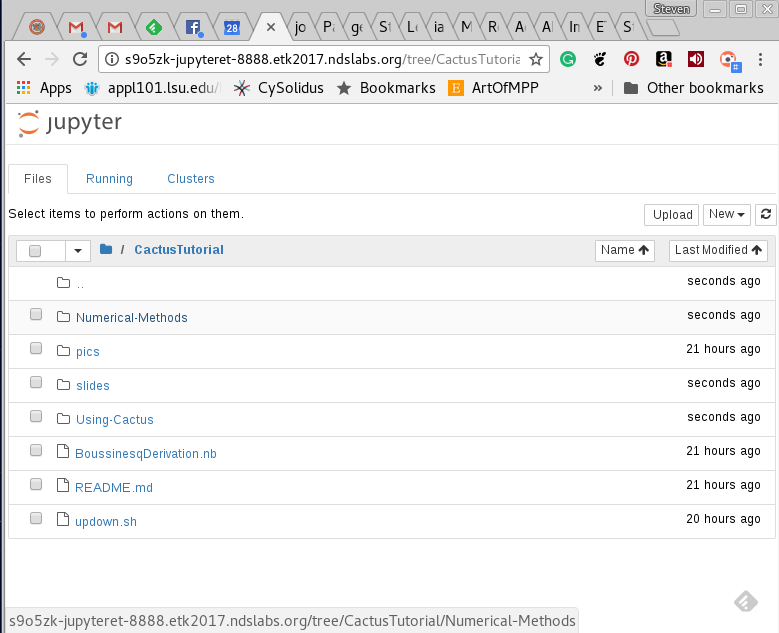
\includegraphics[height=0.45\textwidth]{numerical}\\
\end{centering}
}

\frame{\frametitle{Your Jupyter Notebook}
Now you should see the tutorial materials. Please
click on 01-finite-differencing.ipynb

\begin{centering}
  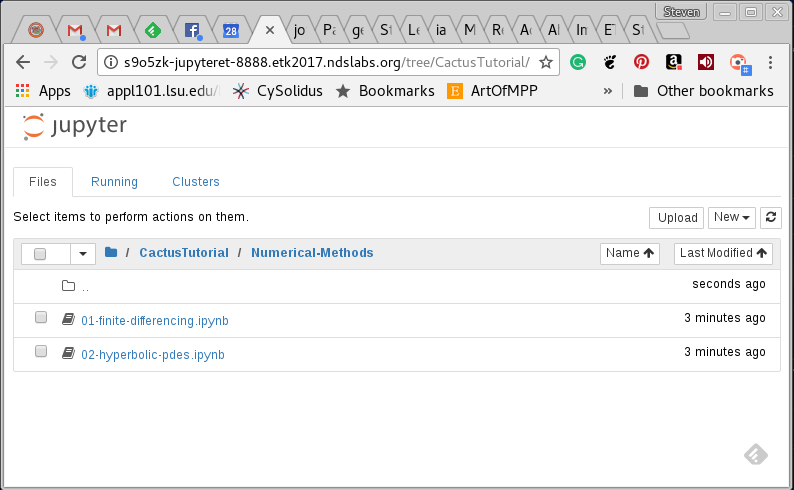
\includegraphics[height=0.45\textwidth]{lesson01}\\
\end{centering}
}

%\frame{\frametitle{Your Jupyter Notebook}
%Click inside the first cell as shown. Hit shift-enter
%to evaluate the cell. Evaluate the next one as well.
%The text ``python 2.7.13'' should print below it.

%\begin{centering}
%  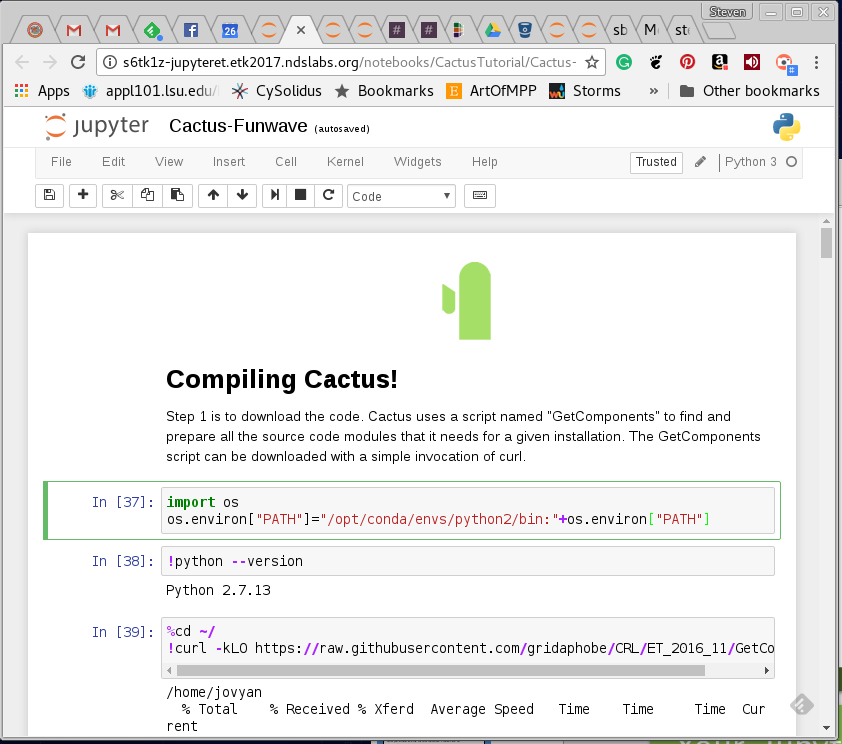
\includegraphics[height=0.45\textwidth]{noteb}\\
%\end{centering}
%}

\frame{\frametitle{Your Jupyter Notebook}
{\huge Your Jupyter Notebook:\\ Basic Commands}
\begin{itemize}
\item \textbf{Python} python commands can be typed interactively.
\item \textbf{Bash} Lines beginning with a ! are shell commands.
\item \textbf{Magics} Certain command start with a \% do special things.
  A handful of these will be used in the presentation.
  \begin{itemize}
  \item \textbf{\%load filename} This command will load the contents of filename
    into the current cell. Once it is loaded, a comment symbol is prefixed in
    front of \%load.
  \item \textbf{\%\%writefile filename} This command will save the contents of
    the current cell (not including the first line) into the named file. By combining
    this and the \%load command, you can use your Juypter notebook as a text editor.
  \end{itemize}
\end{itemize}
}

\frame{\frametitle{Your Jupyter Notebook}
{\huge Your Jupyter Notebook:\\ Basic Commands}
\begin{itemize}
\item To create a new cell, click on ``Insert $>$ Insert Cell Above'' or
``Insert $>$ Insert Cell Below.''.
\item To change a cell type from Code to Markdown, click on the selector
 box at the top of the page. The markdown is quite sophisticated. Any
 text between \$ symbols will be interpreted as latex math code.
\item Be aware that the notebook autosaves. Don't count on changes not
 being made until you explicitly select ``File $>$ Save and Checkpoint.''
 If you want to keep things the way they are, use ``File $>$ Make a Copy.''
\item Don't count on autosaves either. Periodically save your work
with ``File $>$ Save and Checkpoint.''
\end{itemize}
}

\end{document}

